\section{Příklad 2}
% Jako parametr zadejte skupinu (A-H)
\druhyZadani{G}
\subsection{Výpočet Re}
\begin{figure}[H]
    \centering
    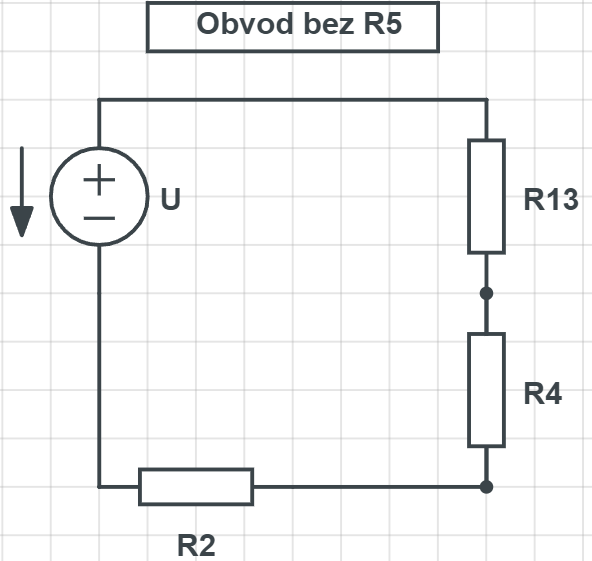
\includegraphics[scale=0.5]{pic2/u2o1.png}
    \caption{Seriove zapojeni $R_1 \: a \: R_3$}
    \label{fig:Serial_resistor_R13}
    \begin{quote}
    \centering
    $R_{13} = R_1 + R_3$ \\~\\
    $R_{13} = 250\Omega + 615\Omega = 865\Omega$
    \end{quote}
\end{figure}
\begin{figure}[H]
    \centering
    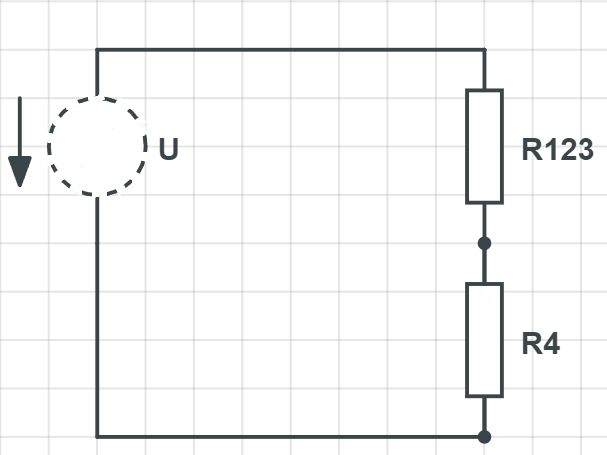
\includegraphics[scale=0.5]{pic2/u2o2.png}
    \caption{Seriove zapojeni $R_{13} \: a \: R_2$}
    \label{fig:Paralel_resistor_R123}
    \begin{quote}
    \centering
    $R_{345} = R_{13} + R_2$ \\~\\~\\
    $R_{345} = 865\Omega + 250\Omega = 1180\Omega$
    \end{quote}
\end{figure}

\begin{figure}[H]
    \centering
    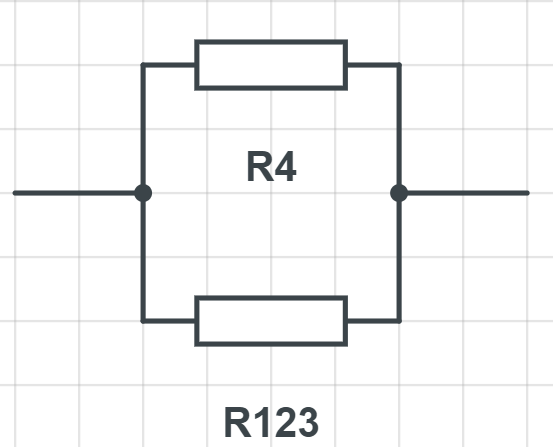
\includegraphics[scale=0.5]{pic2/u2o3.png}
    \caption{Paralelne zapojeni $R_{123} \: a \: R_4$}
    \label{fig:Paralel_resistor_R1234}
    \begin{quote}
    \centering
    $R_e = R_{1234} = \dfrac{R_{123} * R_4}{R_{123} + R_4}$ \\~\\~\\
    $R_e = \dfrac{1180\Omega * 180\Omega}{1180\Omega + 180\Omega} = \dfrac{212 400\Omega}{1360\Omega} = 156.1764\Omega$
    \end{quote}
\end{figure}
\subsection{Výpočet Ue}

\begin{figure}[H]
    \centering
    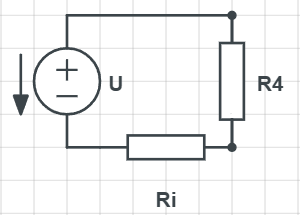
\includegraphics[scale=0.9]{pic2/u2o3.5.png}
    \begin{quote}
        \centering
	    Vypočítáme pomocí napětoví děliče \\~\\ 
	    $U_e = U * \dfrac{R_4}{R_4 + R_{123}} $ \\~\\
	    $U_e = 180\Vo * \dfrac{180\Omega}{180\Omega + 1180\Omega}  = 
	    180\Vo * \dfrac{180\Omega}{1360\Omega} = 23.8235\Vo$ \\~\\
	   
    \end{quote}
\end{figure}

\subsection{Výpočet $U_{R5} \: a \: I_{R5}$}

\begin{figure}[H]
    \centering
    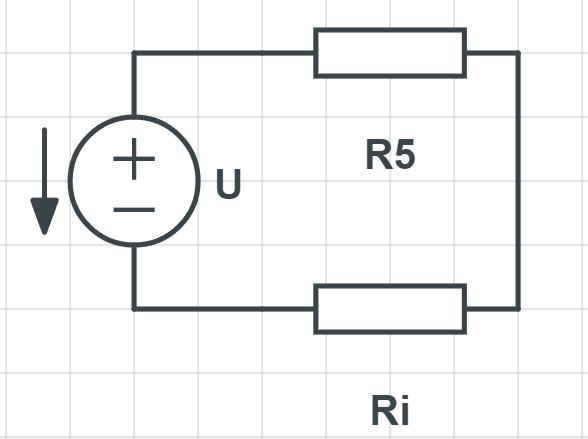
\includegraphics[scale=0.5]{pic2/u2o4.png}
    \begin{quote}
        \centering
	   $I_{R5} = \dfrac{U_e}{R_5 + R_e} = \dfrac{23.8235\Vo}{460\Omega + 156.1764\Omega}
	   = \dfrac{23.8235\Vo}{616.1764\Omega} = 0.0386635\Am$ \\~\\
	   $U_{R5} = R_5 * I_{R5} = 460\Omega * 0.0386635\Am = 17.7852\Vo$
    \end{quote}
\end{figure}